\documentclass{article}
\usepackage[utf8]{inputenc}
\usepackage{tikz}
\usetikzlibrary{positioning}
\usepackage{amsmath}
\usetikzlibrary{arrows,decorations.markings}
\usepackage{amssymb}
\usetikzlibrary{shapes.geometric, arrows}
\title{Proof Diagrams Bessmertnyi}
\author{Anthony Stefan}
\date{September 2020}
\begin{document}
\begin{figure}
\begin{center}
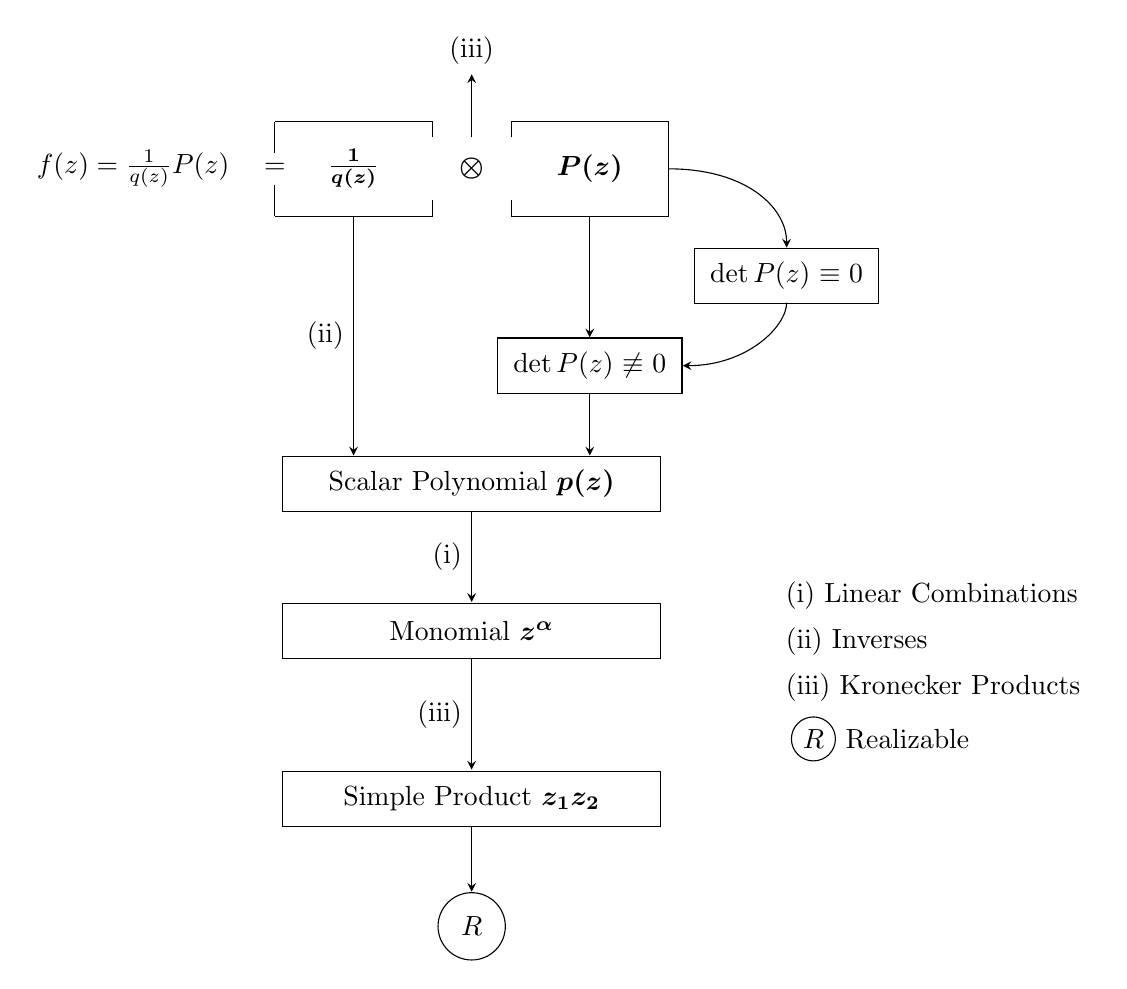
\begin{tikzpicture}[scale=1, %can scale the whole picture once its in our paper
transform shape,
blockone/.style ={rectangle, draw, text width=6em,align=center, minimum height=2em},
blocktwo/.style ={rectangle, draw, text width=13em,align=center, minimum height=2em},
R/.style ={draw, circle, inner sep=5pt},
Rk/.style ={draw, circle, inner sep=2pt}
]
%top equation
\path (0,0) node(x) {$=$}
(-1.8,0) node[](fz) {$f(z) = \frac{1}{q(z)}P(z)$}
(1,0) node[very thick](q/z) {$\boldsymbol{\frac{1}{q(z)}}$}
(2.5,0) node[](kp) {$\boldsymbol{\otimes}$}
(4,0) node[](Pz) {$\boldsymbol{P(z)}$};
%iii arrow
\draw (2.5,1.2) coordinate (iii) node[above] {(iii)};
\draw[->,>=stealth] (2.5,.4) -- (2.5,1.2);
%box above 1/q(z)
\draw (0.0,0.2) coordinate (1);
\draw (0.0,0.6) coordinate (2);
\draw (2,0.4) coordinate (3);
\draw (1) -- (2);
\draw (2) -| (3);
%box under 1/q(z)
\draw (0.0,-0.2) coordinate (1);
\draw (0.0,-0.6) coordinate (2);
\draw (2,-0.4) coordinate (3);
\draw (1) -- (2);
\draw (2) -| (3);
%box of P(z)
\draw (3,0.4) coordinate (4);
\draw (3,0.6) coordinate (5);
\draw (5,-0.6) coordinate (6);
\draw (3,-0.4) coordinate (7);
\draw (4) -- (5);
\draw (5) -| (6);
\draw (6) -| (7);
%qz to scalar poly, pz
\draw (1,-0.6) coordinate (8);
\draw (1,-3.64) coordinate (9);
\draw[->,>=stealth] (8) -- node[left] {(ii)} (9);
%det equal to 0 to invertable to scalar poly pz
\draw (6.5,-1.36) node[blockone] (detzero) {$\det P(z) \equiv 0$};
\draw (4,-2.5) node[blockone] (detnzero) {$\det P(z) \not \equiv 0$};
\draw[->,>=stealth] (5,0) .. controls (6,0) and (6.5,-0.5) .. (6.5,-1);
\draw[->,>=stealth] (6.5,-1.7) .. controls (6.5,-2) and (6,-2.5) .. (5.18,-2.5);
%to invertable
\draw (4,-.6) coordinate (10);
\draw (4,-2.14) coordinate (11);
\draw[->,>=stealth] (10) -- (11);
\draw (4,-2.85) coordinate (12);
\draw (4,-3.64) coordinate (13);
\draw[->,>=stealth] (12) -- (13);
%scalar poly pz
\draw (2.5,-4) node[blocktwo] (sp) {Scalar Polynomial $\boldsymbol{p(z)}$};
%monomial
\draw (2.5,-4.35) coordinate (14);
\draw (2.5,-5.5) coordinate (15);
\draw[->,>=stealth] (14) -- node[left] {(i)} (15);
\draw (2.5,-5.87) node[blocktwo] (m) {Monomial $\boldsymbol{z^{\alpha}}$};
%simple product
\draw (2.5,-6.22) coordinate (16);
\draw (2.5,-7.63) coordinate (17);
\draw[->,>=stealth] (16) -- node[left] {(iii)} (17);
\draw (2.5,-8) node[blocktwo] (z1z2) {Simple Product $\boldsymbol{z_1z_2}$};
%Realizable
\draw (2.5,-8.35) coordinate (18);
\draw (2.5,-9.18) coordinate (19);
\draw[->,>=stealth] (18) -- (19);
\draw (2.5,-9.62) node[R] (R) {$R$};
% Key
\matrix [right] at (6,-6) {
  \node [label=right:(i) Linear Combinations ] {}; \\
  \node [label=right:(ii) Inverses] {}; \\
  \node [label=right:(iii) Kronecker Products] {}; \\
};
\draw (6.84,-7.24) node[Rk] [label=right: Realizable] {$R$};
\end{tikzpicture}
\caption{Proof Flow Diagram \qquad \enspace} 
\end{center}
\end{figure}
\end{document}